\documentclass[onecolumn,12pt]{article} % Documento en dos columnas y tamaño de fuente 12pt
\setlength{\headheight}{14.49998pt}
\usepackage[utf8]{inputenc} % Codificación en UTF-8
\usepackage{amsmath,amsfonts,amssymb} % Paquetes matemáticos
\usepackage{graphicx} % Para incluir imágenes
\usepackage{cite} % Gestión de referencias
\usepackage{geometry} % Configuración de márgenes
\usepackage{microtype}
\usepackage{verbatim}
\setlength{\textwidth}{6.5in}
\usepackage{fancyhdr} % Encabezados personalizados
\usepackage{booktabs}
\usepackage{hyperref} % Enlaces en el documento
\usepackage{pgfplots}
\usepackage{subcaption}
\usepackage{array}
\usepackage{xcolor}
\usepackage{siunitx}
\usepackage{float}
\usepackage[spanish]{babel}
\addto\captionsspanish{\renewcommand{\tablename}{Tabla}}
\usepackage{graphicx}
\usepackage{eso-pic} % Para colocar imágenes absolutas
\pgfplotsset{compat=1.18}
% Márgenes del documento
\geometry{top=2.5cm,bottom=2.5cm,left=2.5cm,right=2.5cm}
\usepackage{tikz}
\usetikzlibrary{shapes.geometric, arrows}

\tikzstyle{startstop} = [rectangle, rounded corners, minimum width=3cm, minimum height=1cm,text centered, draw=black, fill=red!30]
\tikzstyle{process} = [rectangle, minimum width=3cm, minimum height=1cm, text centered, draw=black, fill=blue!30]
\tikzstyle{decision} = [diamond, minimum width=3cm, minimum height=1cm, text centered, draw=black, fill=green!30]
\tikzstyle{arrow} = [thick,->,>=stealth]

% Encabezado personalizado
\pagestyle{fancy}
\fancyhead[L]{\nouppercase} 
\fancyhead[C]{} % Encabezado central
\fancyhead[R]{\today} % Encabezado derecho con la fecha actual




% === Agregar imagen en el borde izquierdo de la página ===
\AddToShipoutPictureBG*{%
  \put(0,0){
\includegraphics[height=\paperheight]{portada.png}} % Cambia el nombre del archivo aquí
}

\usepackage{tocloft} % Permite personalizar el índice
\renewcommand{\cfttoctitlefont}{\Huge\bfseries} % Cambia el tamaño del título del índice


\begin{document}

\thispagestyle{empty}

\begin{flushright}
    \vspace*{0.7cm}

    {\LARGE \textbf{MÁSTER EN}}\\
    {\LARGE \textbf{FÍSICA NUCLEAR}}\\[2cm]

    {\LARGE \textbf{DESARROLLO DE }}\\[0.3cm]
    {\LARGE \textbf{DOSIMETRIA PARA}}\\[0.3cm]
    {\LARGE \textbf{PROTONTERAPIA}}\\[3cm]

    {\Large \textbf{Autor:}}\\
    {\large LUIS FERNANDO HORTA CAMACHO}\\[1.5cm]

    {\Large \textbf{Director:}}\\
    {\large BELÉN CORTÉS LLANOS}\\[0.5cm]

    {\Large \textbf{Co-Director:}}\\
    {\large PABLO DE LA FUENTE FERNÁNDEZ}\\[0.5cm]

    {\Large \textbf{Tutor Académico:}}\\
    {\large CÉLIA TAVARES DE SOUSA}\\[2cm]

    {\Large \textbf{Lugar de realización:}}\\
    {\large CENTRO DE MICROANÁLISIS DE LA MATERIA}\\[3cm]

    {\large \textbf{Trabajo Fin de Máster. Curso 2024 -- 2025}}
\end{flushright}

\newpage % Nueva página después de la portada
\thispagestyle{empty} %
\mbox{} % Espacio vacío para generar la página en blanco
\newpage % Nueva página para continuar el contenido

% Generar el índice
\tableofcontents
\newpage % Empieza una nueva página después del índice

\subsection*{Motivación}

El uso de películas radiocrómicas representa una técnica ampliamente empleada en el ámbito de la investigación para medir la dosis absorbida por tejidos, cultivos celulares u objetos de interés. Esta metodología se vuelve especialmente útil en entornos donde no se dispone de equipamiento especializado propio de la medicina nuclear, ya que permite una estimación fiable y precisa de la dosis entregada durante un proceso de irradiación.

Actualmente, en el \textit{Centro de Microanálisis de Materiales (CMAM)}, se utiliza un software específico para la lectura de las películas radiocrómicas transcurridas 24 horas desde su exposición. Dichas películas son escaneadas mediante un escáner convencional EPSON, y los datos obtenidos se analizan posteriormente con este software. Sin embargo, el proceso de escaneo y análisis puede resultar poco intuitivo y algo laborioso, lo que dificulta su implementación rutinaria, especialmente en contextos donde se requieren múltiples mediciones en tiempos reducidos.

Por ello, uno de los objetivos motivacionales de este trabajo es contribuir a la optimización del software ya existente, con el fin de agilizar el análisis y mejorar la experiencia del usuario. Asimismo, se propone explorar la viabilidad del uso de un fotoespectrómetro como herramienta alternativa para la lectura de las películas radiocrómicas. Este enfoque permitiría reducir considerablemente los tiempos de medición, incrementar la precisión espectral y facilitar la adquisición de datos de forma más automatizada y eficiente.




\subsection*{Objetivos}
\begin{itemize}
    \item Estudiar la bibliografía relacionada con técnicas dosimétricas, tanto en el ámbito clínico como en el de la investigación.

    \item Realizar dosimetría utilizando películas radiocrómicas: emplear y desarrollar un software de medición que permita mejorar y optimizar las herramientas actualmente utilizadas en los experimentos de protonterapia llevados a cabo en el \textit{Centro de Microanálisis de Materiales (CMAM)}.

    \item Investigar y evaluar el uso de técnicas espectrométricas para la lectura de películas radiocrómicas, como una alternativa a los métodos convencionales de medición.
\end{itemize}





\section{Introducción}
\subsection{Interacción de la radiación con la materia.} \label{subsec:interacción}
%En el año 1895, Wilhelm Conrad Röntgen, experimentando con tubos de vacío, descubre los rayos X, obteniendo una imagen del interior del cuerpo humano. De esta manera, abre un campo importante para la ciencia, con aplicaciones en la medicina y en la industria. En un principio, solo se usaba para radiografías, pero posteriormente se fue abriendo paso al comercio.



Dentro del espectro de la radiación ionizante, es posible encontrar distintos tipos de partículas, cada una con características propias que determinan su comportamiento al interactuar con la materia. Estas incluyen partículas cargadas masivas, como protones e iones, partículas cargadas ligeras, como electrones y positrones,  y partículas neutras, como fotones y neutrones. Cada una de estas partículas posee ventajas y limitaciones específicas, tanto en términos de penetración como de capacidad de ionización, lo que influye en su aplicación en áreas como la medicina, la física nuclear y la protección radiológica.

A continuación, se describen los principales mecanismos mediante los cuales la radiación ionizante interactúa con la materia, procesos fundamentales para comprender su efecto biológico y su aprovechamiento en distintas tecnologías.


\subsubsection{Interacción de los fotones con la materia.}
Los fotones tienen diversos mecanismos para interactuar con la materia, como por ejemplo a bajas energías esta Rayleigh y Thomson los cuales no se abordaran en este trabajo.  Mientras que a altas energías existen tres que son los más importantes en el proceso de ionización: el efecto fotoeléctrico, el efecto Compton y la producción de pares.

\subsubsection*{Efecto fotoeléctrico}
Cuando en la materia inciden fotones con energías entorno a unos  cuantos eV hasta unos 100 keV, interactúan con electrones de  capas mayoritariamente externas \cite{fotoelectrico}, cediéndole toda su energía a estos electrones, electrones que escapan del material a los cuales se les conoce como fotoelectrones.  La energía del foto electrón esta dada por :
\begin{equation}
    K_{e^-}=hv-\Phi 
\end{equation}
En donde $hv$ es la energía del fotón incidente y $\Phi $ es la  función de trabajo (o energía de enlace) del electrón en la capa atómica considerada.
\subsubsection*{Efecto Compton}
 El fotón incidente con energías desde 0.01 MeV hasta 10 MeV (dependiendo del material como se puede ver en la figura \ref{fig:seccionefi})  interacciona con un electrón del medio, siendo dispersado un  angulo $\theta$ respecto a la dirección original de propagación (ver figura \ref{fig:compton}), transfiriéndole una  porción de su energía al electrón\cite{Podgorsak2005}. La energía del fotón eyectado y la del electrón Compton están dadas por:
\begin{align*}
    E_{K}&=hv\frac{\varepsilon(1-\cos(\phi))}{1+\varepsilon(1-\cos(\phi))}\\
    hv'&=hv\frac{1}{1+\varepsilon(1-\cos(\phi))}\\
    cot(\theta)&=(1+\epsilon) tan(\phi/2)
\end{align*}
En donde $h\nu$ es la energía del fotón incidente $\varepsilon =\; {h\nu_{0}}/{m_{0} c^{2}}$, y  $ m_{0}c^{2} $ es la energía en reposo del electrón (0.511 MeV).En este proceso tenemos que al final resulta con menor energía el fotón y el electrón con mayor energía.  
\begin{figure}[H]
    \centering
    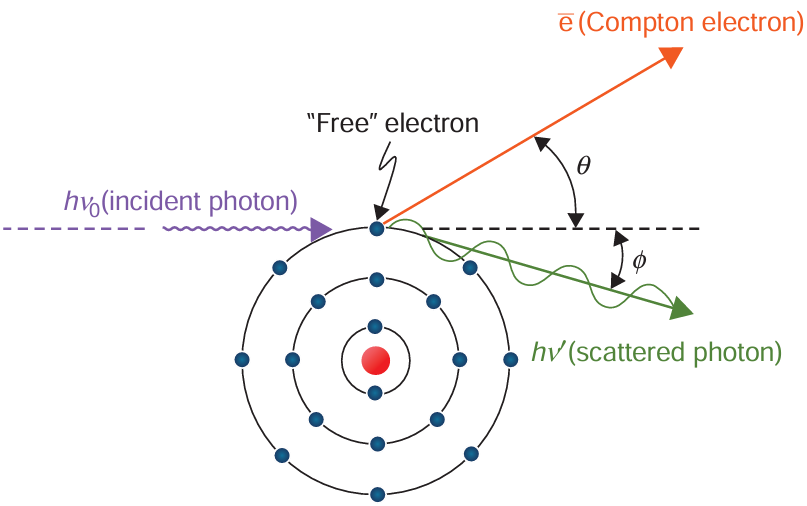
\includegraphics[width=0.5\linewidth]{img_intro/efectoCompton.png}
    \caption{Representación gráfica del efecto Compton}
    \label{fig:compton}
\end{figure}


\subsubsection*{Producción de pares}
En el caso en donde el fotón incidente tiene una energía superior al doble de la masa en reposo del electrón es decir, esta tiene el umbral es de $2m_ec^2$, y el fotón interactúa con el campo Coulombiano del núcleo,  son producidos un par electrón positrón con una energía de $hv-2m_ec^2$ en donde la energía sobrante es repartida en energía cinética en las dos partículas.\cite{Podgorsak2005}
\begin{figure}[H]
    \centering
    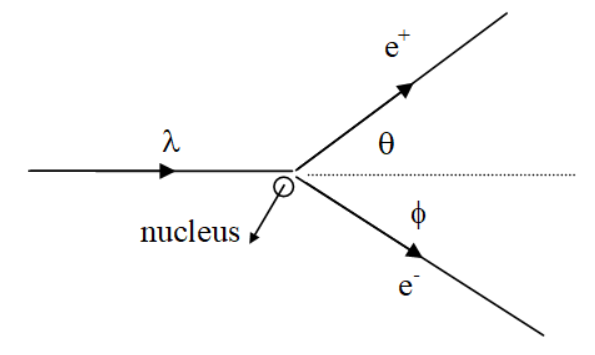
\includegraphics[width=0.5\linewidth]{img_intro/proPares.png}
    \caption{Representación gráfica del proceso de producción de par electrón-positrón}
    \label{fig:proPares}
\end{figure}


No todas las interacciones ocurren siempre, cada una tiene un rango de energías especifico, y no todas se dan de igual manera en todos lo elementos. De la figura \ref{fig:seccionefi} se aprecian las tres secciones en donde es posible que ocurran, estas se dividen en por $\sigma=\tau$ que ocurre cuando la sección eficaz del efecto foto eléctrico es igual a la sección eficaz del efecto Compton, del mismo modo para la linea de $\sigma=\kappa$ ocurren cuando las secciones eficaces del efecto Compton y la producción de pares son iguales. 
\begin{figure}[H]
    \centering
    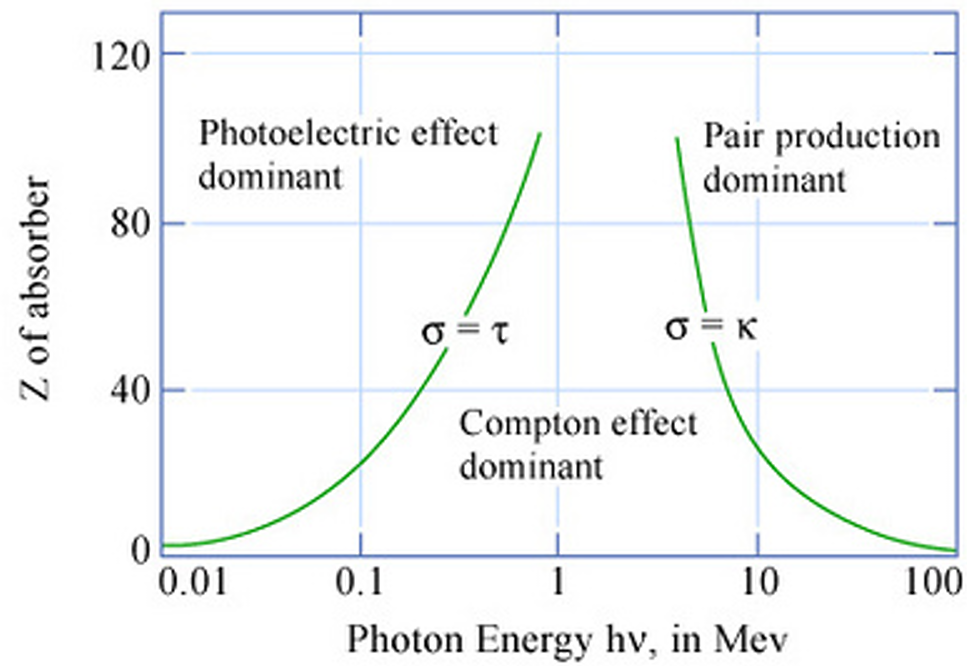
\includegraphics[width=0.5\linewidth]{img_intro/seccionesEficacesDeLasInteracciones.png}
    \caption{Rangos de energía para los diferentes tipos de interacción del fotón con la materia, para diferentes elementos.}
    \label{fig:seccionefi}
\end{figure}



\subsubsection{Interacción de los neutrones con la materia.}
Dado que los neutrones no poseen un campo de fuerza Coulombiano como las partículas cargadas, su interacción con la materia puede ocurrir principalmente de dos formas: mediante \textbf{colisiones}, que generan retrocesos, especialmente con átomos ligeros como el hidrógeno (debido a la similitud de masas) o con núcleos más pesados; y a través de  \textbf{desintegraciones nucleares}, donde el neutrón es capturado por un núcleo atómico, desestabilizándolo y provocando su desintegración.\\

\noindent La primera forma de interacción puede imaginarse como una colisión de esferas  de billar, donde la transferencia de energía es más eficiente cuando las masas de las partículas son similares. Por otro lado, si el neutrón impacta contra un núcleo mucho más pesado, pierde muy poca energía y continúa su trayecto. Debido a esto, materiales densos como el plomo son poco efectivos para atenuar neutrones; en cambio, es recomendable utilizar materiales ricos en hidrógeno, como el polietileno. En cuanto a la dosis producida por un haz de neutrones, esta proviene mayoritariamente del retroceso de los protones generados en las colisiones. Además, las reacciones nucleares inducidas por neutrones generan partículas cargadas adicionales, rayos gamma y otros neutrones, contribuyendo al aumento de la dosis total absorbida en el tejido.





\subsubsection{Interacción de partículas cargadas con la materia.}
Dentro de las partículas cargadas se encuentran los electrones, positrones, protones, iones y partículas alfa. Estas partículas interactúan con la materia principalmente a través de dos mecanismos: la \textbf{ionización} y la \textbf{excitación}.
\\
En el proceso de \textit{ionización}, un electrón es removido de un átomo, dejando a este último en un estado ionizado. El electrón liberado se desplaza a través del medio, con la posibilidad de interactuar con otros electrones y depositar la energía adquirida. Posteriormente, el átomo ionizado puede capturar un electrón del entorno para regresar a su estado neutro.

Por otro lado, la \textit{excitación} ocurre cuando un electrón de un átomo absorbe energía y es promovido a un nivel de energía superior. Eventualmente, el electrón regresa a su órbita original, liberando la energía absorbida en forma de un fotón.
\subsubsection*{Electrones y Positrones}

Las interaciones de un electron con la materia se dan por medio de su campo Coulombiano, este interacciona con el campo de los electrones orbitales y el núcleo de  los átomos de la materia. Dada estas interacciones el electrón puede perder su energía cinética  por medio de colisiones  y perdías radiactivas, o también puede cambiar su trayectoria y dispersarse. 

La energía inelástica perdida por un electrón en movimiento a través de un medio material con densidad $\rho$ se describe mediante el \textit{poder de frenado}, el cual representa la energía cinética que pierden los electrones por unidad de longitud recorrida $x$.  \cite{Podgorsak2005}.


\begin{equation}
    \left( \frac{S}{\rho} \right)_{\text{tot}} = \frac{1}{\rho} \, \frac{dE_K}{dx} \quad \left( \si{\mega\electronvolt\cdot\centi\meter\squared\per\gram} \right)
\end{equation}

en donde $(S/\rho)_{tot}$ tiene dos componentes;  el poder de frenado másico $(S/\rho)_{col}$, que es el resultado de  las interacciones de los electrones con los electrones del orbital, y $(S/\rho)_{rad}$  que es el poder de frenado radiactivo, resultado de la interacción electrón núcleo. En el primero ocurren eventos como las excitaciones atómicas y las ionizaciones, y en el segundo la producción de bremsstrahlung.

\begin{equation*}
    (S/\rho)_{tot}=(S/\rho)_{col}+(S/\rho)_{rad}
\end{equation*}

El termino $(S/\rho)_{tot}$ es de gran importancia en  dosimetria, dado que expresamos la dosis $D$ en el medio por medio de $D=\phi(S/\rho)_{col}$ en donde $\phi$ es la fluencia de electrones. Este termino se puede ver con mas claridad en la ecuación \ref{ecu:poderdefrenado}. 
 



Por otro lado, el positrón, tiene la misma masa que el electrón, 0.511 MeV/c\(^2\), con la misma carga \(1.602 \times 10^{-19}\) C, pero opuesta a la del electrón. 

Los positrones al igual que los electrones interactúan por medio del campo electromagnético, sin embargo estos  al ser antipartículas, sus trayectorias  varían,  y pueden ocurrir aniquilaciones, en donde un positron choca con un electrón y libera 1.022 Mev en forma de dos fotones. Esta ultima es de alta importancia en física medica, ya que por medio del  decaimiento \(\beta^+\) son utilizados en la tomografía por emisión de positrones (PET, por sus siglas en inglés). Este método nos permite observar de manera clara el interior del cuerpo en áreas específicas, al introducir un fármaco como el Flúor-18 que se acumula en regiones del cuerpo con alta actividad metabólica. Esto hace posible realizar un diagnóstico temprano de cáncer, llevar a cabo monitoreos de respuesta a tratamientos oncológicos y mucho más. 







\subsubsection*{Partículas pesadas}
Se considera partícula pesada a partículas que se sean mucho más grandes que el electrón, como los protones e iones. Los cuales son producidos en aceleradores de partículas. Las principales partículas pesadas que se maneja en física medica están dadas por:


\begin{table}[H]
\centering
\begin{tabular}{c c c c c c c}
\toprule
\textbf{Átomo} & \textbf{Símbolo} & \shortstack{ \textbf{Abundancia}\\ \textbf{natural (\%)}} & \shortstack{ \textbf{Nombre}\\ \textbf{(núcleo)}} &
\textbf{p} &
\textbf{n} &
\shortstack{ \textbf{Estabilidad}\\ \textbf{nuclear}} \\
\midrule
\hline
Hidrógeno-1 & \( ^1_1\text{H} \) & 99.985 & Protón & 1 & 0 & Estable \\
Hidrógeno-2 & \( ^2_1\text{H} \) & 0.015 & Deuterón & 1 & 1 & Estable \\
Hidrógeno-3 & \( ^3_1\text{H} \) & – & Tritón & 1 & 2 & Radiactivo \\
Helio-3     & \( ^3_2\text{He} \) & 0.00014 & Helión & 2 & 1 & Estable \\
Helio-4     & \( ^4_2\text{He} \) & 99.99986 & Partícula alfa & 2 & 2 & Estable \\
Carbono-12  & \( ^{12}_6\text{C} \) & 98.93 & – & 6 & 6 & Estable \\
Carbono-14  & \( ^{14}_6\text{C} \) & – & – & 6 & 8 & Radiactivo \\
Oxígeno-16  & \( ^{16}_8\text{O} \) & 99.76 & – & 8 & 8 & Estable \\
Oxígeno-18  & \( ^{18}_8\text{O} \) & 0.20 & – & 8 & 10 & Estable \\
\bottomrule
\end{tabular}
\caption{Propiedades básicas de partículas cargadas pesadas utilizadas en física nuclear y medicina \cite{podgorsak2022}.}
\end{table}

La tasa de energía perdida por la partícula a través del medio, también conocida como \textit{stopping power} (poder de frenado), causada por la ionización de las partículas cargadas, es proporcional a  la carga de la partícula e inversamente proporcional a la raíz de su velocidad. Esto quiere decir que, a medida que las partículas van perdiendo energía, van ionizando aún más el medio, por lo que la dosis absorbida aumenta. La fórmula de Bethe-Bloch que representa el tasa de energía transferida esta dada por:
\begin{equation}
- \left\langle \frac{dE}{dx} \right\rangle = \frac{4\pi}{m_e c^2} \cdot \frac{z^2 e^4}{\beta^2} \cdot \frac{Z}{A} \cdot \rho \cdot \left[ \ln\left( \frac{2 m_e c^2 \beta^2 \gamma^2}{I} \right) - \beta^2 \right]
\label{ecu:poderdefrenado}
\end{equation}

En donde; $m_e$ masa del electrón, $c$ velocidad de la luz en vació, $z$ numero atómico del proyectil, $e$ carga electrón,  $\beta$ velocidad relativista del proyectil, $\gamma$ es el factor relativista, $Z$ numero atómico del material blanco, $A$ numero  másico del material blanco, $\rho$ densidad del blanco, $I$ energía media necesaria para ionizar el blanco.  

Si se gráfica este comportamiento, se observa que al principio la dosis absorbida es bastante baja, hasta que se alcanza un punto donde aparece un pico muy pronunciado en el cual se deposita casi toda la dosis. A esto se le conoce como el \textit{pico de Bragg}, el cual abordaremos con mas detalle en la siguiente sección (figura \ref{fig:bragg_peak}). 


Como se ha visto a lo largo de esta sección , la manera en que interactúan las partículas masivas con la materia es a través de varios procesos, depositando energía en el medio a lo largo de su trayectoria.  Esta transferencia de energía es medible y se conoce como \textbf{LET} (\textit{Linear Energy Transfer}), aunque puede confundirse con la pérdida de energía o \textbf{poder de frenado} (\textit{stopping power}). La diferencia radica en que el poder de frenado incluye la energía que se pierde por la radiación, es decir, por la producción de partículas secundarias con energía relativamente alta que recorren distancias significativas, y también la energía que se pierde por las interacciones con los electrones (ionizaciones). Mientras que  el LET representa la pérdida de energía de un haz de radiación al atravesar un espesor dx de material, pero en este caso se refiere únicamente a la pérdida de energía debido a las interacciones con electrones (ionizaciones). Dado que en medicina es necesario saber el daño biológico producido por la reacción, se usa el LET, ya que mide la energía de las ionizaciones producidas localmente.  En otras palabras :
\begin{equation}
    L_{\Delta} = S_{\text{el}} - \frac{dE_{\text{ke},\Delta}}{dl}.
\end{equation}
en donde $L_{\Delta}$ es LET, $S_{\text{el}}$ poder de frenado eléctrico, y $\frac{dE_{\text{ke},\Delta}}{dl}$ es la tasa de perdida de energía asociada a los electrones secundarios con energía mayor a  $\Delta$. 








\section{Protonterapia} 

A la hora de tratar el cáncer, la medicina cuenta con diversos métodos, como lo es la medicina  interna o externa. En el caso de la medicina interna  consiste en el uso de fármacos radiactivos que se incorporan al cuerpo para irradiar las células tumorales desde el interior. La otra opción es emplear haces de partículas externos, como fotones, electrones o protones. En ambos casos —ya sea mediante medicina interna o externa— el objetivo de la irradiación es dañar el ADN de las células tumorales para provocar su muerte y evitar que se sigan duplicando.\cite{Podgorsak2005}
 \\




La tasa de pérdida de energía por ionización y excitación causada por una partícula cargada al atravesar un medio es proporcional al cuadrado de su carga e \textbf{inversamente proporcional al cuadrado de su velocidad}. A medida que la partícula pierde energía, su velocidad disminuye, lo que incrementa la tasa de pérdida de energía por unidad de longitud recorrida. Cuando la velocidad de la partícula se aproxima a cero, cerca del final de su recorrido, esta tasa alcanza su valor máximo.  Este fenómeno se puede explicar considerando que, cuando la partícula cargada pierde energía cinética, las demás partículas comienzan a experimentar  su campo Coulombiano y son repelidas o atraídas por este, lo que provoca una mayor actividad en esa región \cite{khan}

La distribución de dosis en profundidad refleja este comportamiento. En el caso de un haz de protones monoenergético, se observa inicialmente un aumento gradual de la dosis con la profundidad, seguido por un incremento abrupto cerca del final de su alcance. Este aumento pronunciado en la deposición de dosis es  el \textbf{pico de Bragg}. Como se puede apreciar en la figura \ref{fig:bragg_peak}. 
\begin{figure}[H]
    \centering
    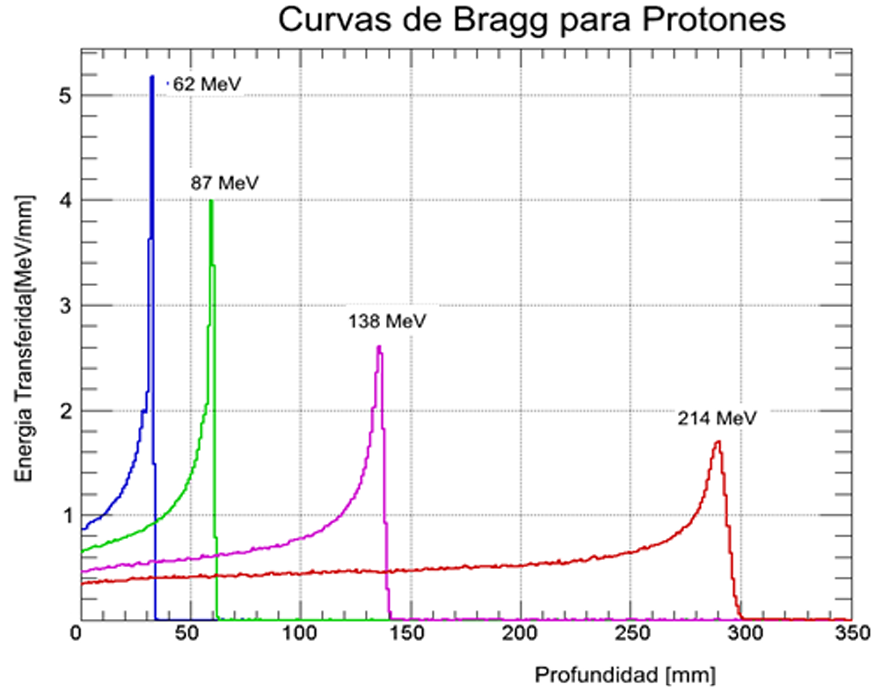
\includegraphics[width=0.6\textwidth]{img_intro/picoBragg.png}
    \caption{\textbf{Distribución de dosis en profundidad sobre el eje central} para un haz de protones a diferentes energías sobre un phantom de agua.\cite{unal2014}}
    \label{fig:bragg_peak}
\end{figure}







\subsection{Ventajas de la Protonterapia.}
El tratamiento del cáncer mediante radioterapia se fundamenta en la capacidad de eliminar las células tumorales minimizando el daño a los tejidos sanos. Esto ha sido posible gracias a los avances tecnológicos, que han permitido el desarrollo de equipos capaces de administrar la dosis con alta precisión en las zonas afectadas.\cite{chen2017titulo}.


Cuando los protones (generalmente en el rango de 70 a 250 MeV) atraviesan un medio, su velocidad disminuye progresivamente a medida que penetran más profundamente. La energía que depositan (el \textit{LET}),  se incrementa conforme su velocidad disminuye, alcanzando un máximo justo antes de detenerse por completo. En ese punto final de su trayectoria es donde liberan la mayor parte de su energía~\cite{jones1999lack}. Según la formula de Bethe-Bloch (ecuacion \ref{ecu:poderdefrenado}) , y modelos analítico  como el propuesto por Bortfeld~\cite{bortfeld1997}, la dosis absorbida guarda una relación inversa con la energía cinética, y por lo tanto, con el cuadrado de la velocidad.

La manera en que los protones transfieren su energía a los tejidos permite una dosificación precisa a los tumores, minimizando daños en los tejidos sanos colindantes. No obstante, la geometría del paciente, los movimientos internos del cuerpo, y la heterogeneidad de los tejidos atravesados por el haz de protones son problemas significativos en la implementación del tratamiento, y que requieren ser solucionados~\cite{bras2024in}. Por esto, delimitar un margen de tratamiento adecuado se vuelve relevante para la efectividad de la protonterapia, así como para minimizar los efectos secundarios.



\begin{figure}[H]
    \centering
    \begin{subfigure}[b]{0.45\textwidth}
        \centering
        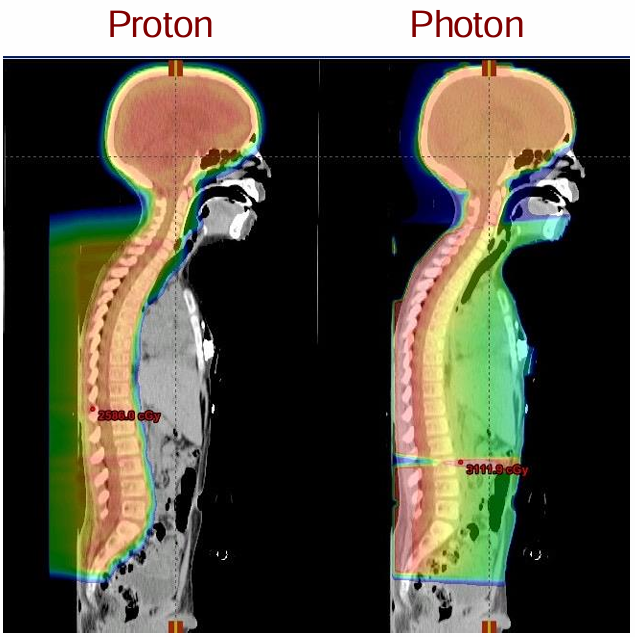
\includegraphics[width=\textwidth]{img_intro/protonterapia.png}
        \caption{Comparativa del tratamiento de meduloblastoma de columna vertebral, usando Protonterapia y radiación convencional}
        \label{fig:medula}
    \end{subfigure}
    \hfill
    \begin{subfigure}[b]{0.5\textwidth}
        \centering
        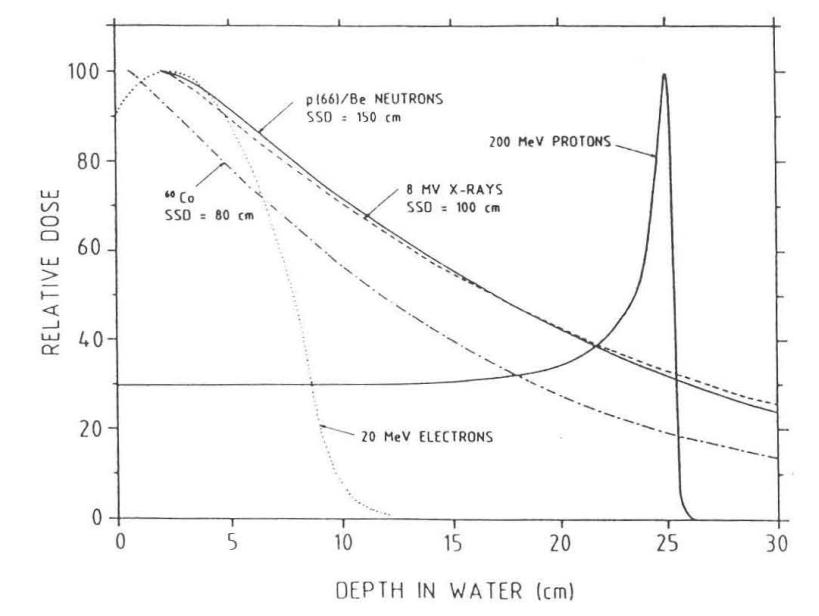
\includegraphics[width=\textwidth]{img_intro/Figura_comparacion_dosis.png}
        \caption{Perfiles de dosis para diferentes tipos de particulas,(66VBe \textit{neutron therapy beam} 200 MeV \textit{proton therapy beam} comparado con haces de radioterapia convencionales }
        \label{fig:picoVarasparticulas}
    \end{subfigure}
    \caption{ Diferencias en el daño de células sanas para dos tipos de haces.}
    \label{fig:diferenciaradioterapia}
\end{figure}

Esta entrega total de la dosis tan focalizada hace que la protonterapia destaque entre entre las otras vías para tratar tumores cancerígenos. Si se desea cubrir un volu



En el estudio de España et al.~\cite{parceriza}, mostraron que el uso de agua-18 (H\textsubscript{2}O con \textsuperscript{18}O) como agente de contraste permite la ejecución de escaneos PET con precisión milimétrica para verificar la extensión del haz en la terapia con protones. Con un modelo tumoral de cabeza y cuello en embriones de pollo, se observó la formación (vía la reacción \textsuperscript{18}O(p,n)\textsuperscript{18}F) y retención de \textsuperscript{18}F, lo que permite estimar el rango del haz a través de imágenes PET fuera de línea. Además, la mayor vida media de \textsuperscript{18}F ayuda en su detección por escáneres PET convencionales libres de otros isótopos interferentes, como se había demostrado en trabajos anteriores~\cite{espana2021}. Estos hallazgos justifican la necesidad de pruebas adicionales con modelos animales más grandes.



% Actualmente las principales vías de desarrollo de la protonterapia son la reducción de costos, la genera lización del brazo isocéntrico, la modulación de intensidad por protones, la reducción de incertitudes en la penetración y la determinación de las localizaciones clínicas las mas adecuadas. Se realizan asimismo un gran número de estudios de radiobiología, micro-haces, alta intensidad y modificadores locales de la acción del haz como el uso de nano-partículas.


 
\subsection{ Métodos y técnica de administración.}
Dentro de los tratamientos de protonterapia que se encuentran en la actualidad, existen dos métodos de administración para los pacientes: dispersión pasiva (Scatter Beam) y escaneo activo o Pencil Beam Scanning (PBS). Dentro de estos, hay varias técnicas de administración, como la convencional, la terapia de protones de intensidad modulada (IMPT) y la terapia FLASH de protones, unas con mas evidencias que otras. 

El método de dispersión pasiva (Scatter Beam), en el cual se emplean láminas metálicas para ampliar su área de irradiación, busca abarcar más el área a tratar. Esto se logra mediante colimadores y ventanas para ajustar un perfil preciso al tumor del paciente.

TERMINAR



\subsubsection{Método Convencional}

\subsubsection{Método Flash}








\subsection{Dosimetria en Protonterapia}
Desde el descubrimiento de la radiación misma es de vital importancia conocer  la cantidad de energía que se deposita en  un cuerpo. Para conocer esta cantidad existen en el mercado diversos métodos dependido de que tipo de radiación  es lo que se requiere en el estudio o tratamiento.

En el caso de la dosimetria hospitalaria tenemos varios detectores como los son las cámaras de ionización, los TLD, los diodos, los MOSFET, los detectores de alanina, los centelleadores plásticos, los detectores de diamante, los dosímetros de luminiscencia ópticamente estimulada (OSLD), los sistemas de dosimetría radiofotoluminiscente (RPL) y los sistemas de dosimetría en gel.





Añadir lo de las técnicas dosimetria tanto en lab como e hospitales, radiocromicas,fotodiodo , faraday caps, RBS. CI.
tambien Añadir la simulacion de topas de cuanta energia es depositada en la capa activa. 
\\


Lo que se esta investigando actualmente en técnicas de dosimetria  tanto clínicas como de investigación.



Una de las estrategias actualmente en estudio consiste en aplicar Protonterapia acompañada de visualización en tiempo real de la zona irradiada. Esta técnica se basa en la generación de isótopos radiactivos mediante el propio haz de protones, permitiendo el análisis de la región tratada mediante imágenes PET (tomografía por emisión de positrones). Sin embargo, presenta limitaciones como la baja intensidad de señal en la región del pico de Bragg y la pérdida de emisores PET debido a la actividad biológica de los tejidos~\cite{parceriza}.




\section{Experimento y toma de datos.}
El presente trabajo  se realizo  conjunto a otra investigación que consiste en la viabilidad del glioblastoma multiforme (GBM) que es el tumor cerebral maligno más frecuente y agresivo en adultos, haciendo incidir en estas células dosis de 0 a 20 Gy, se realizaron varias pruebas, como la viabilidad celular, la generación especies reactivas  de oxigeno (ROS), el ciclo celular y la capacidad clonogénica mediante espectroscopia de fluorescencia.\cite{CIATAR A ....}


\begin{figure}[H]
    \centering
    \begin{subfigure}[b]{0.45\textwidth}
        \centering
        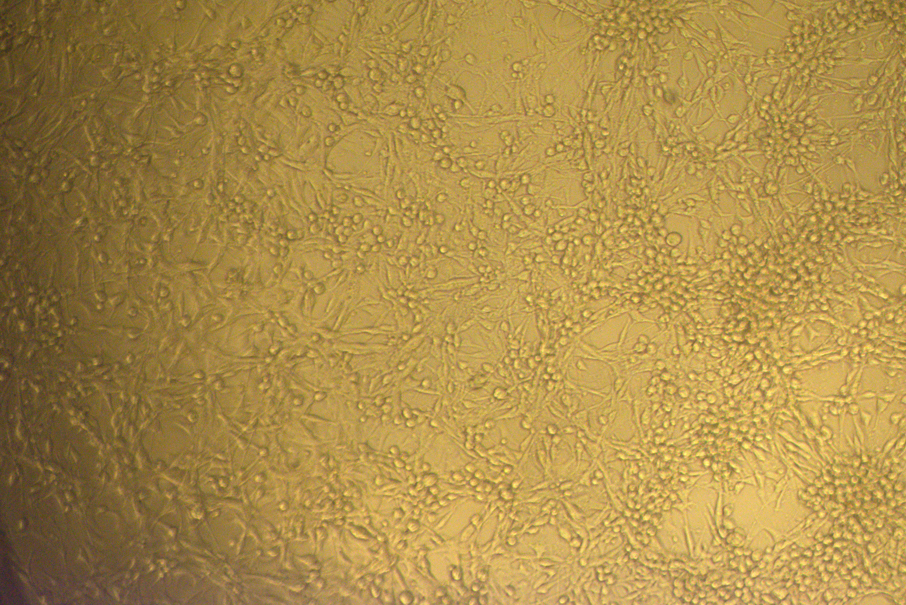
\includegraphics[width=\textwidth]{img_exp/pt2_ct.png}
        \caption{Cultivo celular de glioblastoma multiforme, sin irradiar}
        \label{fig:pt2_ct}
    \end{subfigure}
    \hfill
    \begin{subfigure}[b]{0.5\textwidth}
        \centering
        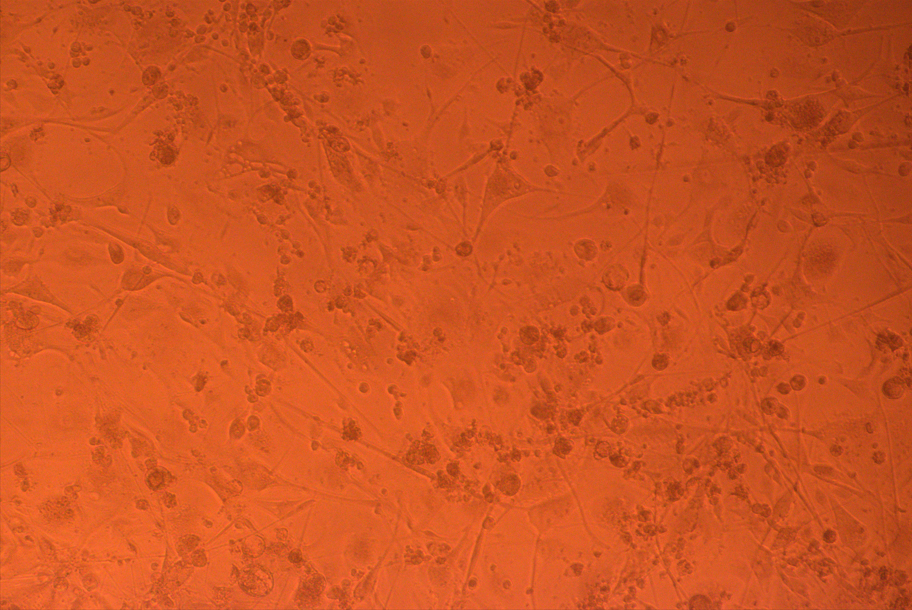
\includegraphics[width=\textwidth]{img_exp/pt2_15gy.png}
        \caption{Cultivo celular de glioblastoma multiforme, irradiado con aproximadamente 15 Gy}
        \label{fig:pt2_15Gy}
    \end{subfigure}
    \caption{Muerte celular para }
    \label{fig:celulas}
\end{figure}


Como se aprecia en las figuras \ref{fig:celulas} el daño causado por la irradiación a las células se evidencia en el hecho de que ya no se ve el mismo numero de colonias por mm cuadrado, y ha perdido la capacidad de multiplicarse. 



\subsection{Calibración radiocrómicas.}

Para el buen uso de las radiocromicas es necesario realizar una calibración que consiste en irradiar una serie de radiocromicas con dosis conocidas y bien definidas con equipo preciso,  de tal manera que al medir los colores por los canales \textbf{RGB} \textit{(Red Green Blue)} se puedan estos ajustar a una curva. 

El procedimiento se realizo en el centro hospitalario Clínica Universidad de Navarra (CUN), el cual posee  un acelerador lineal (LINAC) de electrones. En términos generales este funciona acelerando los electrones por medio de campos electromagnéticos y hacerlos colimar contra un metal pesado, de esta manera que se generen rayos-X de alta energía, rayos que son conducidos hacia el paciente con la forma he intensidad según se requiera. Dado que este equipo es de uso clínico, es ideal para calibrar las RC, dado que tiene ya todo un sistema bastante preciso, de tal forma que nos podamos asegurar que en la capa activa de la RC si se recibe la dosis que se requiere. 

Se hicieron 16 tiras de $1.5 \times 5$ $cm^2$, las cuales se hicieron irradiar con diferentes dosis (ver fig \ref{fig:tonosRC}). Pasadas 24 horas se realiza un escanear de las RC utilizando un equipo EPSON, estos se guardan en formato .tiff con 300 DPI de resolución. Una vez guardados todos los archivos procedemos a realizar la calibración; utilizando un código escrito en  MATLAB,  tomado y modificado de Taylor (Servidor del CMAM), con el consentimiento de Silvia \footnote{\href{silvia.vinnals@inv.uam.es }{silvia.vinnals@inv.uam.es}}. Lo que hacemos con este programa es seleccionar un área de $20\times 20 $ px (ver fig \ref{fig:areatomadaRC}) , buscando siempre el centro de la RC, esto por motivo homogeneidad. 
\begin{figure}[H]
    \centering
    \begin{subfigure}[b]{0.45\textwidth}
        \centering
        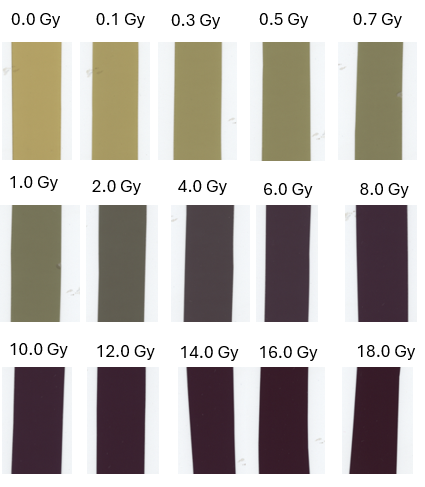
\includegraphics[width=\textwidth]{img_exp/calibracionRC.png}
        \caption{Diferentes tonalidades que toman las radiocromicas a la hora de ser irradiadas con diferentes dosis.}
        \label{fig:tonosRC}
    \end{subfigure}
    \hfill
    \begin{subfigure}[b]{0.5\textwidth}
        \centering
        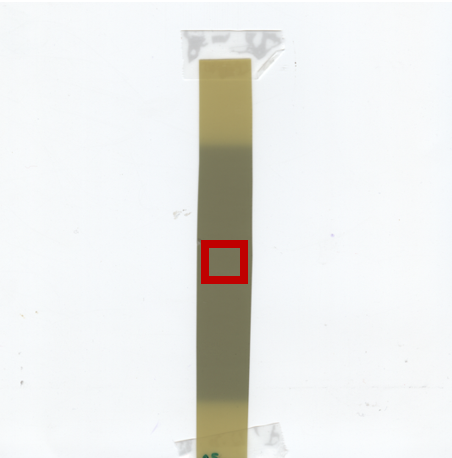
\includegraphics[width=\textwidth]{img_exp/scanCalibRC.png}
        \caption{Área tomada en cada tira de las RC que se usan para calibración}
        \label{fig:areatomadaRC}
    \end{subfigure}
    \caption{Cortes tomados para realizar la correcta calibración  de las RC.}
    \label{fig:calibracionRC}
\end{figure}

Una vez seleccionada el área de todas las radiocromicas y asignarle  la dosis que le corresponde. El código lo que hace es por medio de los canales RGB y usando el residuo cuadrado, 
\begin{equation}
    \bigl[D_i - \mathrm{model}(PV_i; a, b, c)\bigr]^2\, ,
\end{equation}
en donde $D_i$ es la dosis que hemos introducido, de modo que el código busca dentro de nuestro modelo empírico, 

\begin{equation}
    D(Gy) = a + \frac{b}{PV - c} \, ,
\end{equation}
los mejores parámetros a, b, y c. De tal manera que podemos sacar las curvas de calibración (ver fig \ref{fig:curvaCalRC} ), con sus respectivos valores. 
\begin{figure}[H]
    \centering
    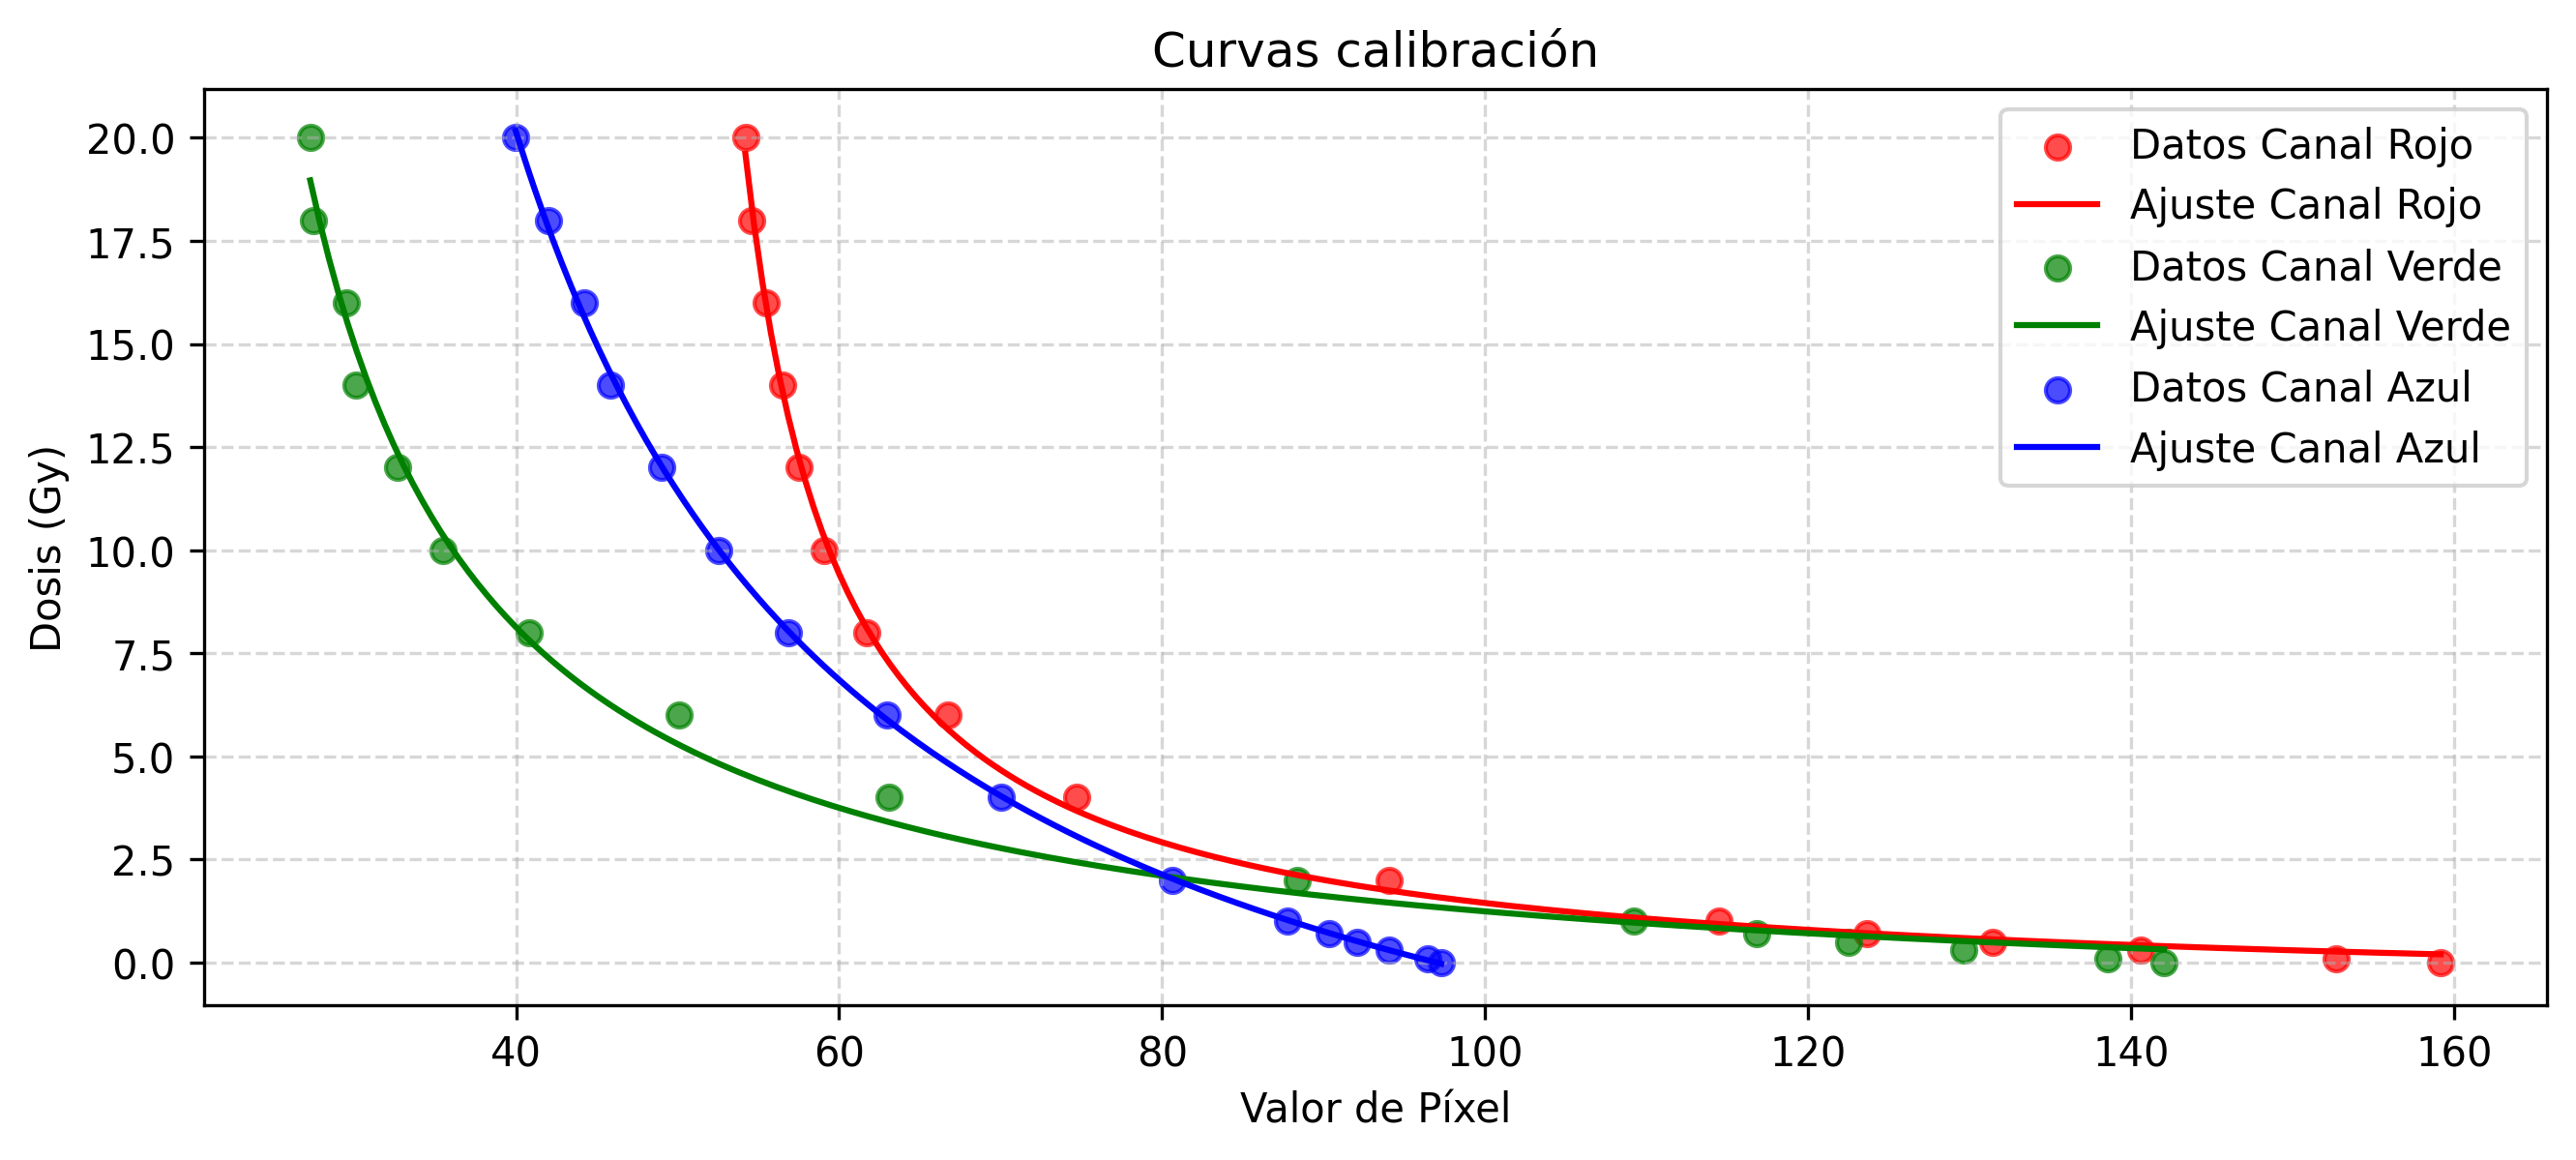
\includegraphics[width=0.7\linewidth]{img_exp/calibration_curves.png}
    \caption{Curvas de calibración de las radiocromicas, en los canales RGB, con un $R^2=0.999$ para los tres canales.} 
    \label{fig:curvaCalRC}
\end{figure}

Los valore obtenidos en la calibración son guardados en un archivo .txt para su posterior uso de las lecturas RC. Los paramtros que se obtuvieron son los siguientes:

\begin{table}[H]
  \centering
  \label{tab:calibracion}
  \begin{tabular}{lrrrr}
    \hline
    \textbf{Canal} & \(\boldsymbol{a}\) & \(\boldsymbol{b}\) & \(\boldsymbol{c}\) & \(\mathbf{95\%\ CI}\) \\
    \hline
    \textcolor{red}{Rojo}   & \(-0.8904\)     & \(120.5440\)   & \(48.3162\)   & \(\pm0.2897,\ \pm10.3384,\ \pm0.5125\) \\
    \textcolor{green}{Verde}& \(-1.5296\)     & \(232.8529\)   & \(15.8913\)   & \(\pm0.7377,\ \pm48.0220,\ \pm2.2564\) \\
    \textcolor{blue}{Azul}  & \(-7.7989\)     & \(616.3912\)   & \(17.9348\)   & \(\pm0.5497,\ \pm47.0843,\ \pm1.3936\) \\
    \hline
  \end{tabular}
  \caption{Parámetros de Calibración}
\end{table}

\subsection{Acelerador lineal tipo TÁNDEM}
El acelerador tipo tándem que posee el centro de micro análisis de materiales (CMAM), alcanza tensiones de hasta 5 MV. 
El funcionamiento principal de este tipo de aceleradores , consiste en  hacer pasar iones con carga negativa por medio de un tramo en donde el campo electromagnético  es negativo, y con un choque en un stripper de gas, el ion pierde los  electrones  por lo que cambia de carga, con carga positiva  ahora es acelerado por un tramo con campo positivo, véase la figura \ref{fig:tandem}.
\begin{figure}[H]
    \centering   
    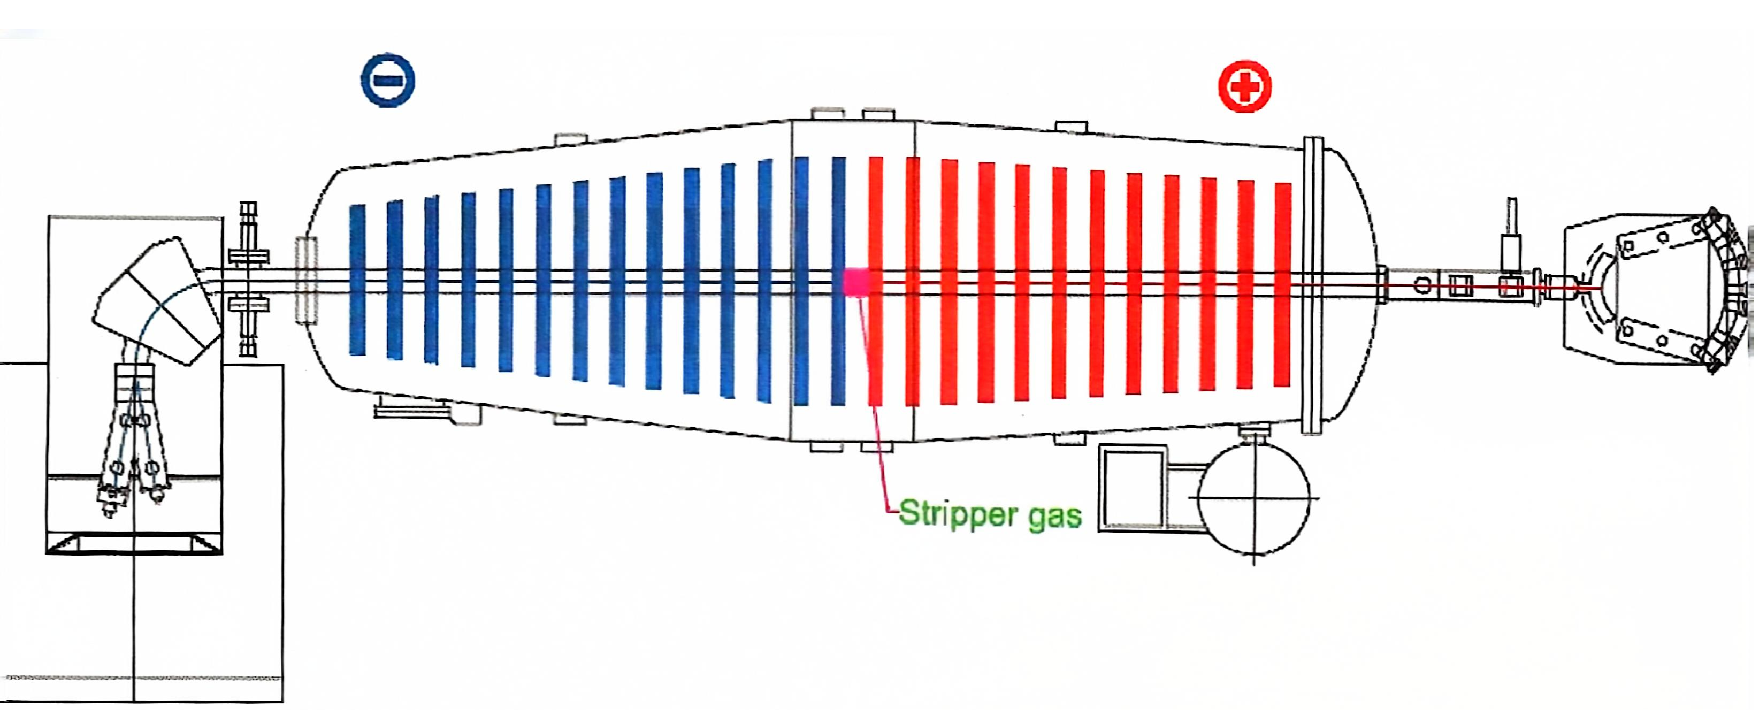
\includegraphics[width=0.6\linewidth]{img_intro/TipoTandem.pdf}
    \caption{Esquema del acelerador tipo tándem del CMAM.}
    \label{fig:tandem}
\end{figure}
Esta aceleración es posible gracias  la Ley de Lorentz, que viene dada por la ecuación \ref{ecu:lorentz}
\begin{equation}
   \vec{F_L} = q \cdot (\vec{E}+v\times\vec{B})
   \label{ecu:lorentz}
\end{equation}

El interior del acelerador aparte de tener sus anillos que generan el campo electromagnético  esta aislado eléctricamente con un gas de hexafluoruro de azufre $(SF_6)$, que tiene una alta rigidez eléctrica, lo que significa que puede soportar altos voltajes sin descomponerse eléctricamente. Además, es químicamente estable y no inflamable.

Las energías que alcanzan los iones son impuestas según el experimento las requiera, y estas vienen dadas por la ecuación \ref{ecu:energia}. 

\begin{equation}
    E=(1+q)V_T
    \label{ecu:energia}
\end{equation}
De esta ecuación podemos apreciar que si utilizamos todo el potencial  del acelerador es decir $V_T= 5$MV, una partícula con carga $q=1$ saldrá con una energía de hasta $10 $MeV. Dado que son varios los usos que se le puede dar un haz de iones con estas energías es posible tener varias lineas experimentales  gracias a un imán de deflexión, en donde  con este  podemos re dirigir el haz. 

\begin{figure}[H]
    \centering
    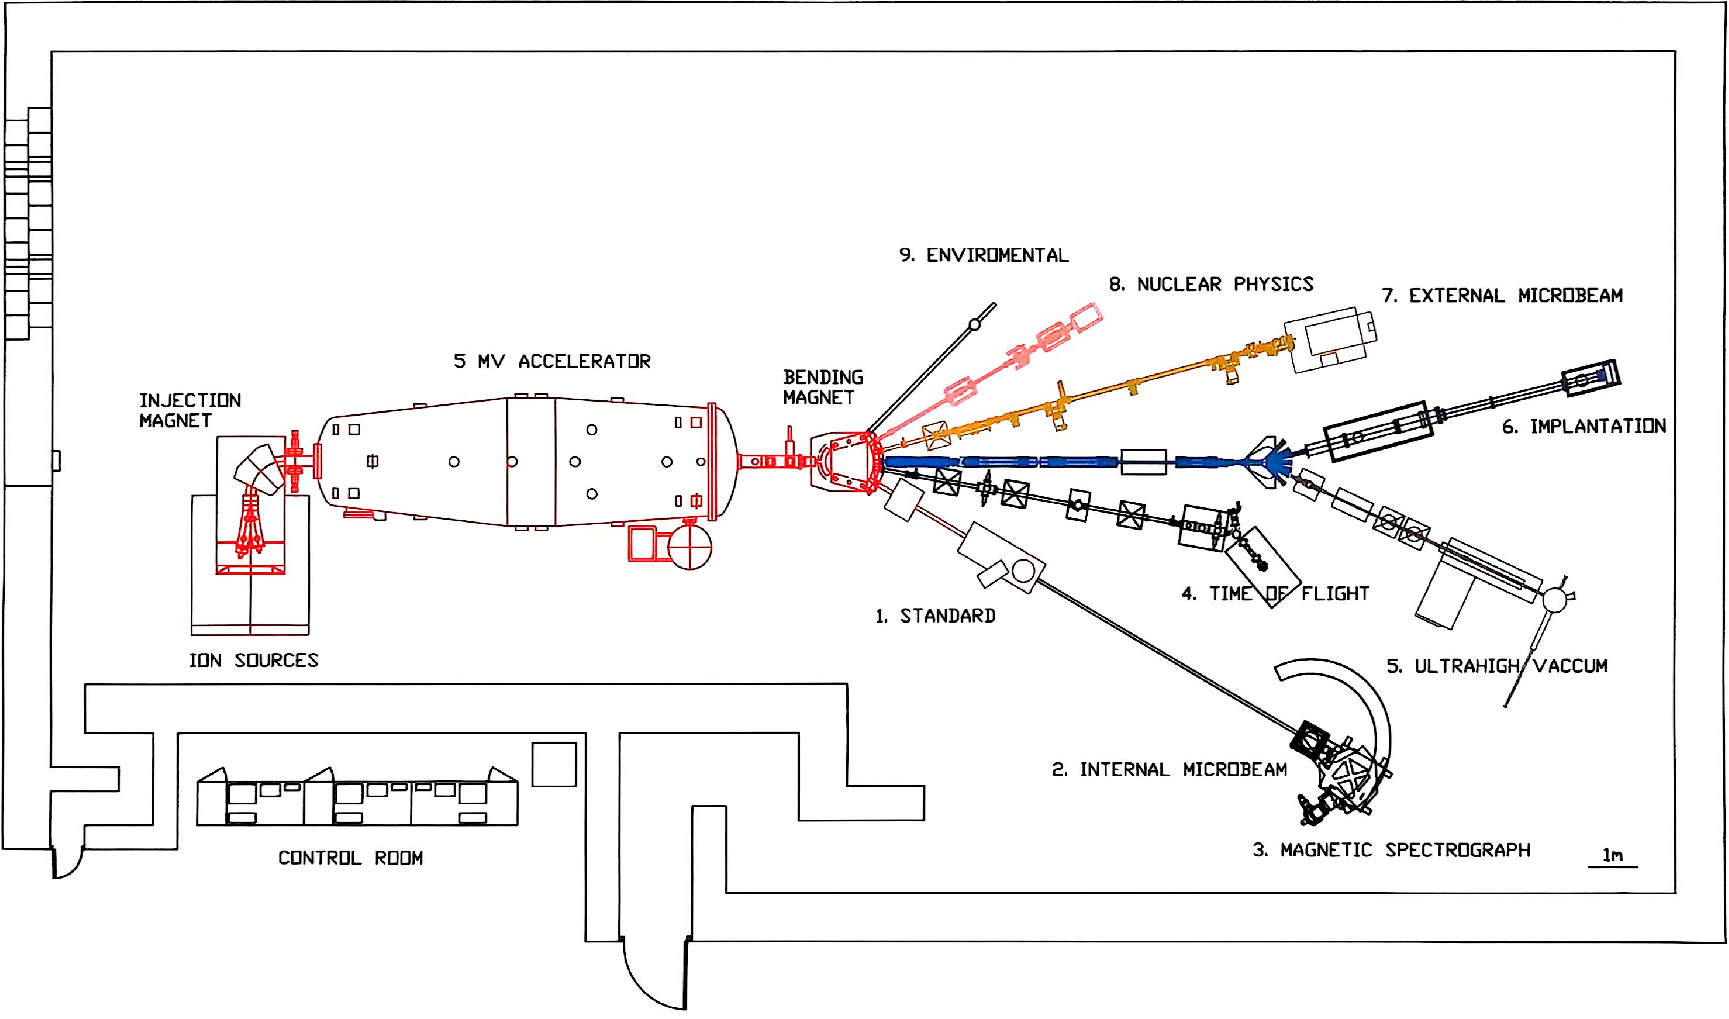
\includegraphics[width=0.5\linewidth]{img_intro/EsquemaAcelerador.pdf}
    \caption{Lineas experimentales del acelerador del CMAM}
    \label{fig:lieasExp}
\end{figure}
En el Centro de Micro-Análisis de Materiales (CMAM) se desarrollan diversas líneas de investigación (véase la Figura~\ref{fig:lieasExp}), cada una con objetivos científicos particulares. El presente trabajo se enmarca dentro de la línea de implantación, cuyo propósito principal es el estudio y la modificación de las propiedades de los materiales mediante técnicas como la implantación iónica, con el fin de alterar sus características eléctricas, ópticas o mecánicas.

Dentro de esta misma línea, también se investiga el efecto de la radiación en sistemas biológicos, especialmente en células, lo cual permite evaluar posibles aplicaciones en campos como la medicina o la biotecnología.

La estación experimental correspondiente se encuentra situada en el puerto $-20^\circ$ del segundo imán de conmutación, el cual está conectado al puerto 0 del acelerador. Esta disposición permite realizar irradiaciones homogéneas sobre superficies de hasta $100,\text{mm} \times 100,\text{mm}$, incluso en condiciones de energía elevada (hasta 10 MeV), gracias a un sistema de raster de haz electrostático rápido (operando a frecuencias del orden de kHz) proporcionado por la empresa HVE.

La cámara de irradiación se encuentra eléctricamente aislada y ha sido diseñada para operar bajo condiciones de ultra alto vacío. El sistema de montaje permite la utilización de obleas de hasta 3 pulgadas de diámetro. La fluencia se controla mediante la medición de la corriente del haz a través de dos métodos complementarios: una copa de Faraday ubicada antes de la válvula de vacío y un conjunto de cuatro copas de Faraday situadas después de dicha válvula e inmediatamente antes de la cámara de irradiación \cite{cmam_uam_2023}.



\begin{figure}[H]
    \centering
    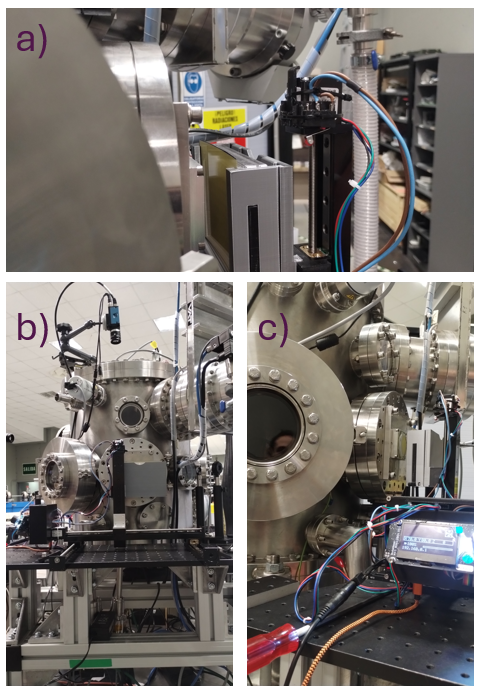
\includegraphics[width=0.5\linewidth]{img_exp/stage.png}
    \caption{a)Vista lateral del brazo del stage portando una radiocromica que apunta a la brida del acelerador, b) Vista panorámica de todo el satge. c) Control del brazo del stage, que es conectado al computador para poder ser manejado remotamente. }
    \label{fig:enter-label}
\end{figure}

\begin{figure}[H]
    \centering
    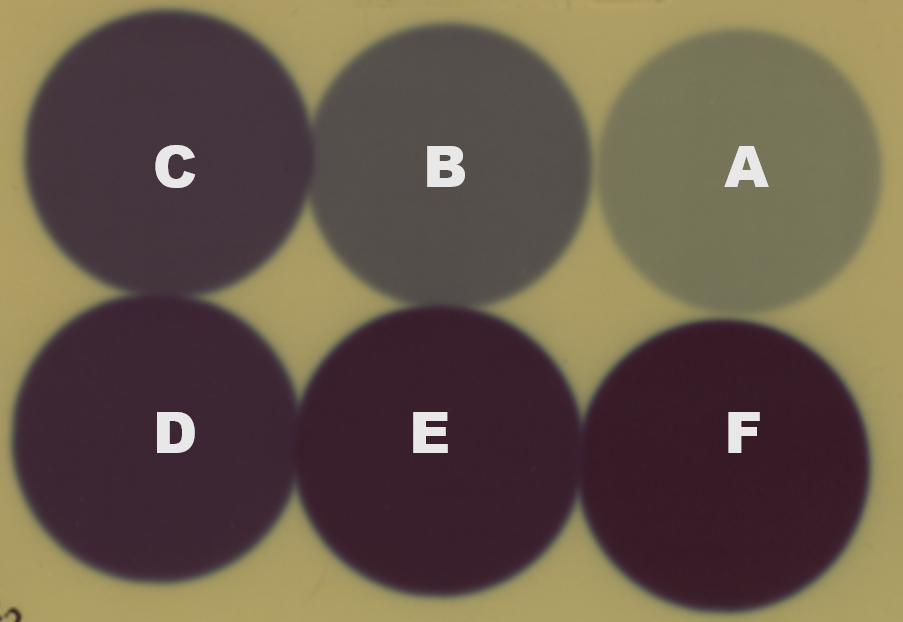
\includegraphics[width=0.7\linewidth]{img_exp/RC_letrada.png}
    \caption{Ejemplo de calibración para un experimento con el acelerador tándem.}
    \label{fig:RCletrada}
\end{figure}



aqui se explica todo lo que se hizo con e en el avance del programa y lo que se realizo con el fotoespectrometro, tambien se debe mensionar los ajustes que se hicieron y por que uno es mejor que otro, lorentz e integral.




















\begin{figure}[H]
    \centering
    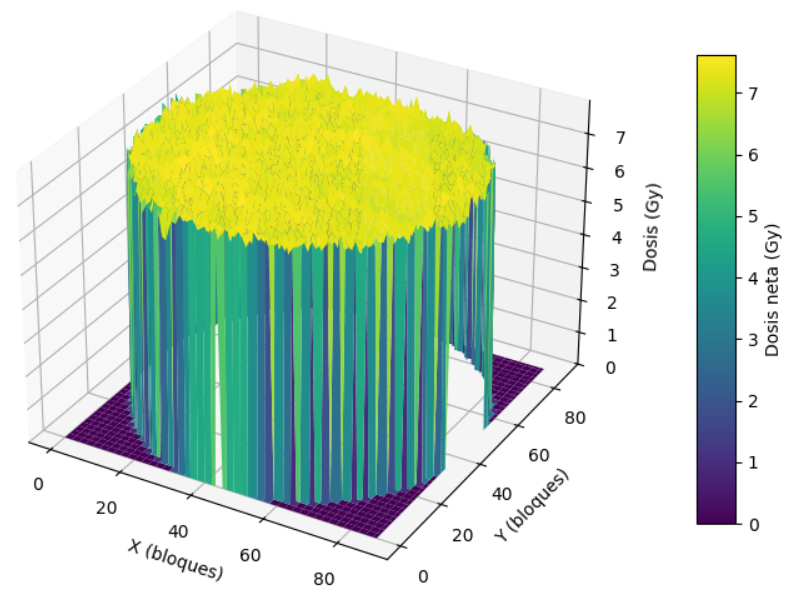
\includegraphics[width=0.5\linewidth]{img_exp/3DConvencional.png}
    \caption{Caption}
    \label{fig:enter-label}
\end{figure}

\begin{figure}[H]
    \centering
    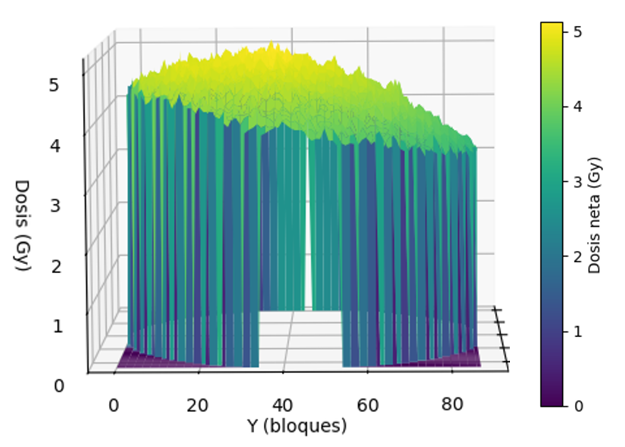
\includegraphics[width=0.5\linewidth]{img_exp/3Dflash.png}
    \caption{Caption}
    \label{fig:enter-label}
\end{figure}

\begin{figure}[H]
    \centering
    \begin{subfigure}[b]{0.45\textwidth}
        \centering
        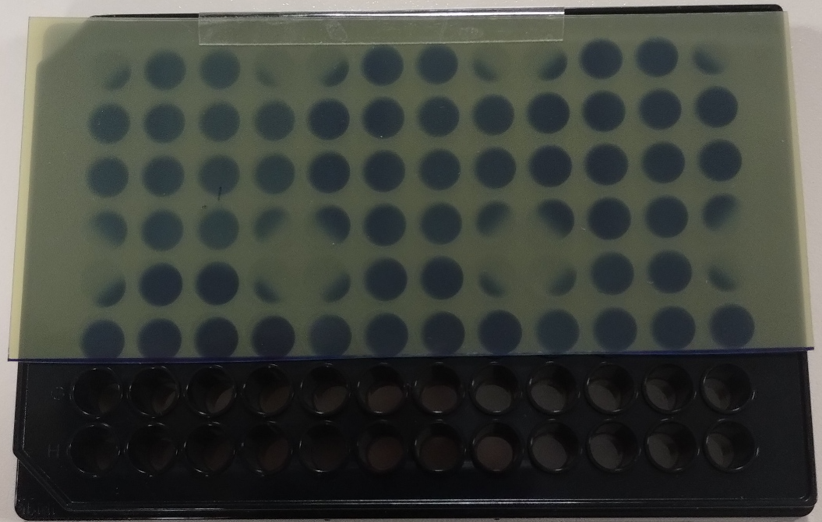
\includegraphics[width=\textwidth]{img_exp/pocillosconRC.png}
        \caption{Descripción imagen 1}
        \label{fig:img1}
    \end{subfigure}
    \hfill
    \begin{subfigure}[b]{0.5\textwidth}
        \centering
        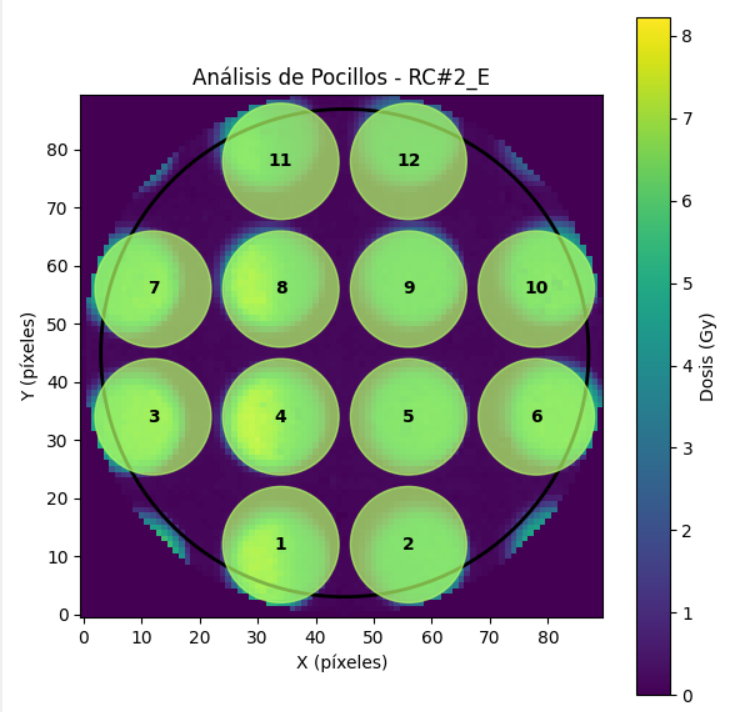
\includegraphics[width=\textwidth]{img_exp/AnaPocillos.png}
        \caption{Descripción imagen 2}
        \label{fig:img2}
    \end{subfigure}
    \caption{Título general para ambas imágenes}
    \label{fig:ambas}
\end{figure}




\subsection{Medición con el espectrofotómetro.}

\begin{figure}[H]
    \centering
    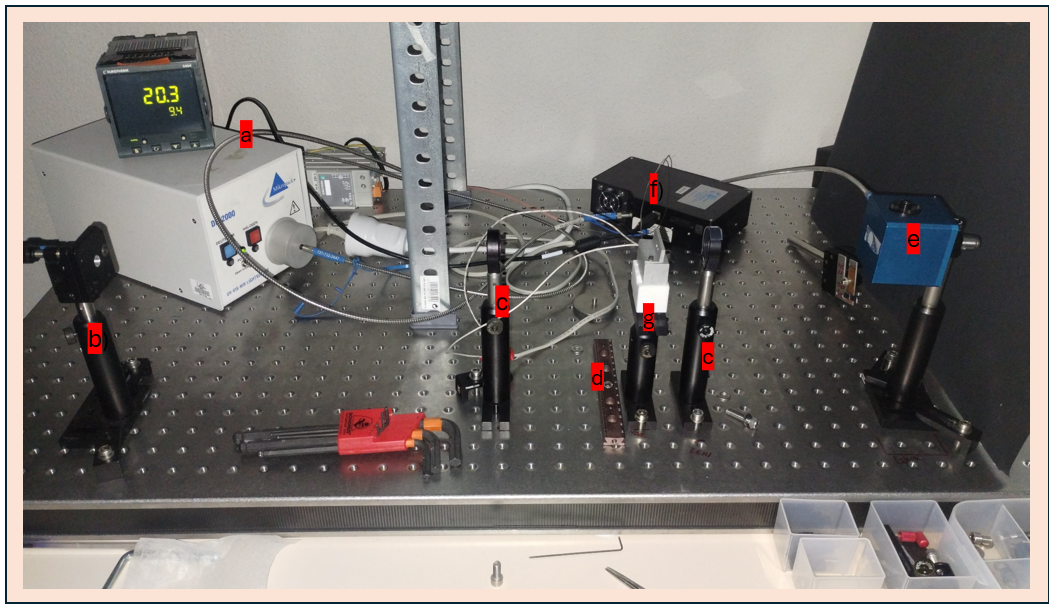
\includegraphics[width=0.7\linewidth]{img_Esp/montaje_espectrometria.png}
    \caption{Montaje experimental usado en la espectrofotómetria de las radiocromicas. \textit{ a) fuente de luz blanca, b) lentes colimadores, c) lentes focales, d) posición de las muestras, e) esfera de integración, f) espectrometro }  }
    \label{fig:setup_esp}
\end{figure}
\begin{equation}
O.D = \log_{10} \left(\frac{I_0}{I}\right)    
\end{equation}

\begin{figure}[H]
    \centering
    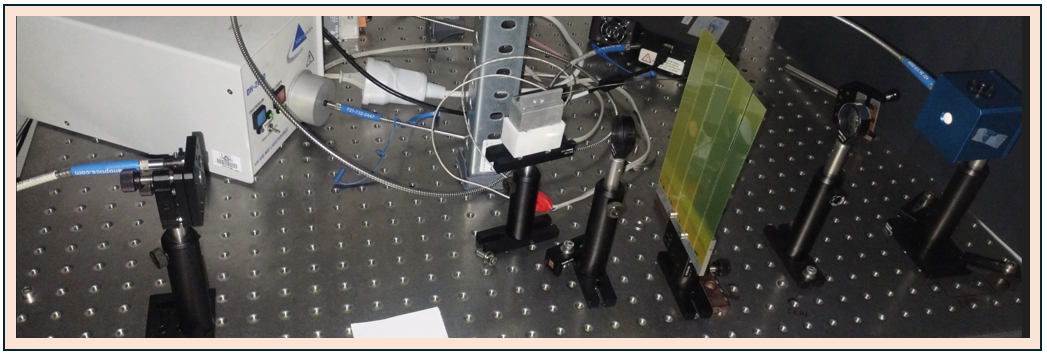
\includegraphics[width=0.7\linewidth]{img_Esp/montaje_espectrometria_conRadiocromica.png}
    \caption{Montaje experimental con las radiocromicas de calibración para ser medidas.}
    \label{fig:setup_espConRC}
\end{figure}



\section{Análisis y resultados}


\subsection{Ajuste Integral}

\begin{figure}[H]
    \centering
    \begin{subfigure}[b]{0.45\textwidth}
        \centering
        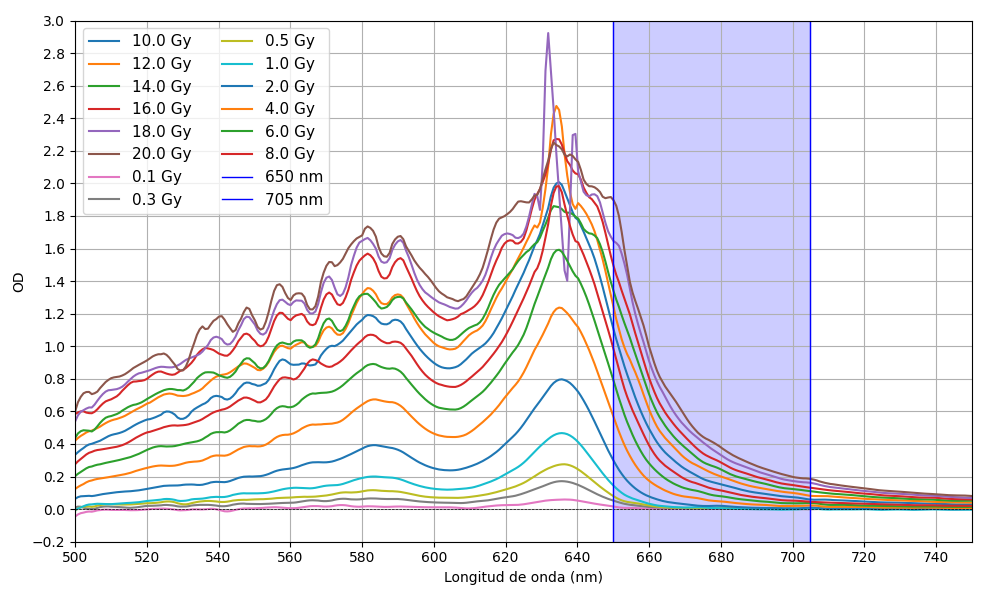
\includegraphics[width=\textwidth]{img_Esp/Integral.png}
        \caption{Descripción imagen 1}
        \label{fig:img1}
    \end{subfigure}
    \hfill
    \begin{subfigure}[b]{0.5\textwidth}
        \centering
        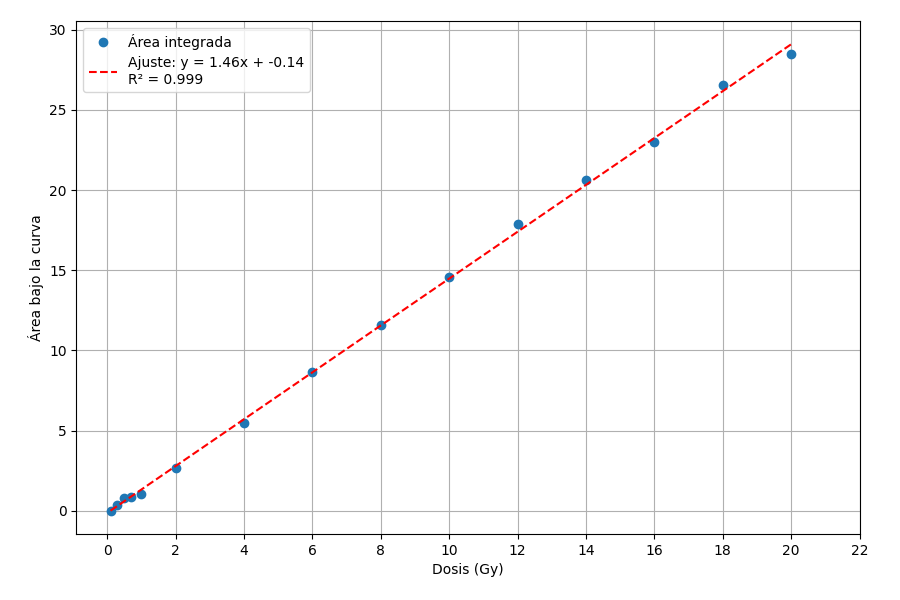
\includegraphics[width=\textwidth]{img_Esp/IntegralCali.png}
        \caption{Descripción imagen 2}
        \label{fig:img2}
    \end{subfigure}
    \caption{Título general para ambas imágenes}
    \label{fig:ambas}
\end{figure}


\subsection{Ajuste Lorentzianas}

\begin{figure}[H]
    \centering
    \begin{subfigure}[b]{0.45\textwidth}
        \centering
        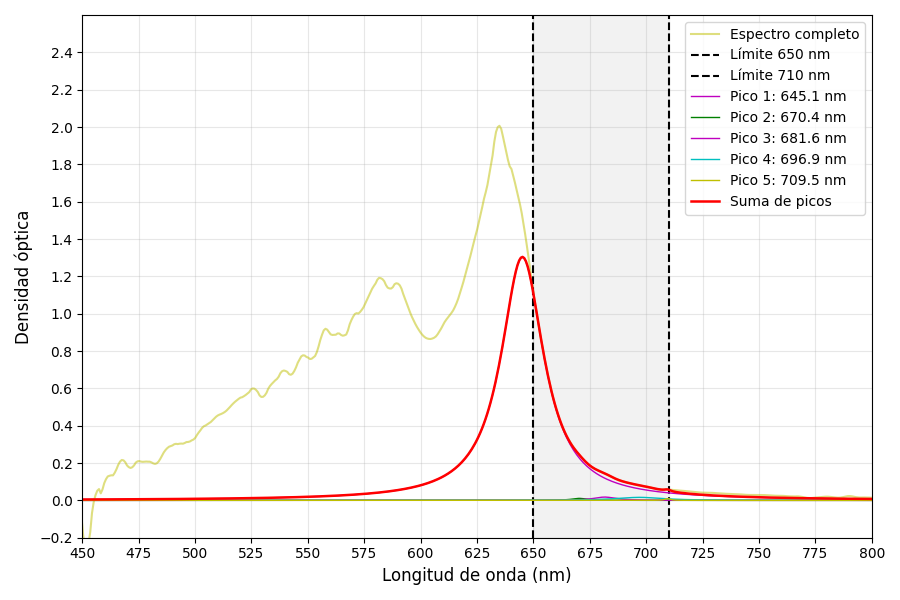
\includegraphics[width=\textwidth]{img_Esp/Lorentz.png}
        \caption{Descripción imagen 1}
        \label{fig:img1}
    \end{subfigure}
    \hfill
    \begin{subfigure}[b]{0.5\textwidth}
        \centering
        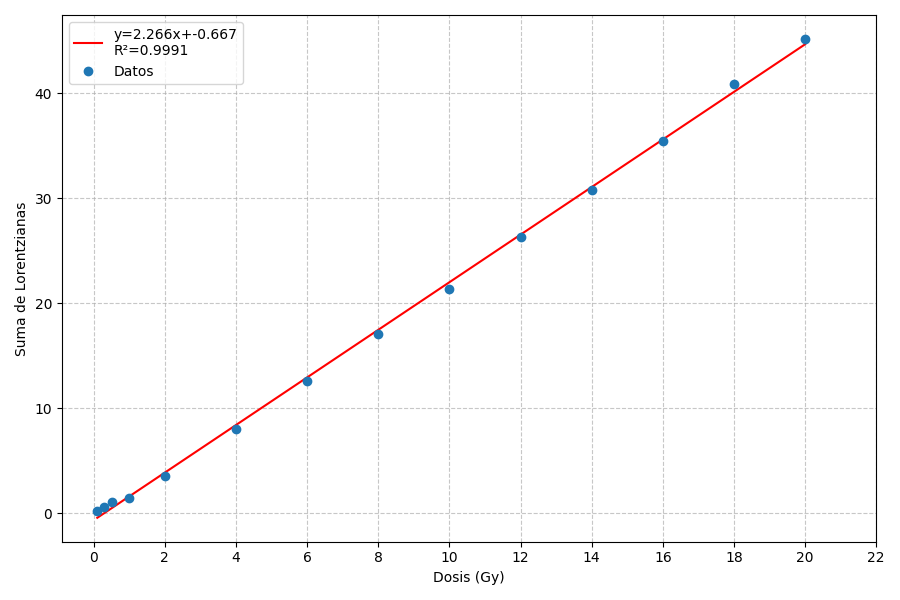
\includegraphics[width=\textwidth]{img_Esp/LorentzCalib.png}
        \caption{Descripción imagen 2}
        \label{fig:img2}
    \end{subfigure}
    \caption{Título general para ambas imágenes}
    \label{fig:ambas}
\end{figure}


\subsection{Ajuste 663 nm}

\begin{figure}[H]
    \centering
    \begin{subfigure}[b]{0.5\textwidth}
        \centering
        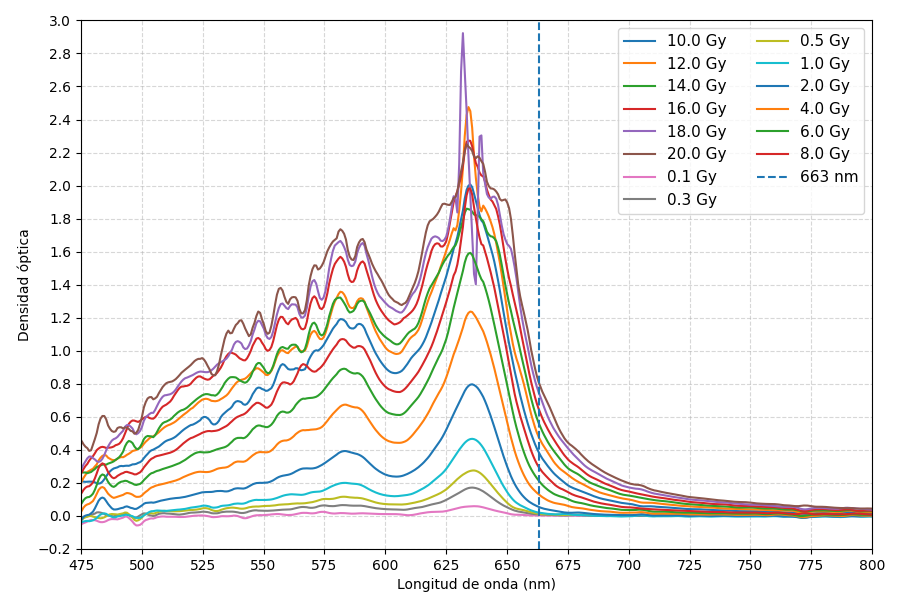
\includegraphics[width=\textwidth]{img_Esp/663.png}
        \caption{Descripción imagen 1}
        \label{fig:img1}
    \end{subfigure}
    \hfill
    \begin{subfigure}[b]{0.5\textwidth}
        \centering
        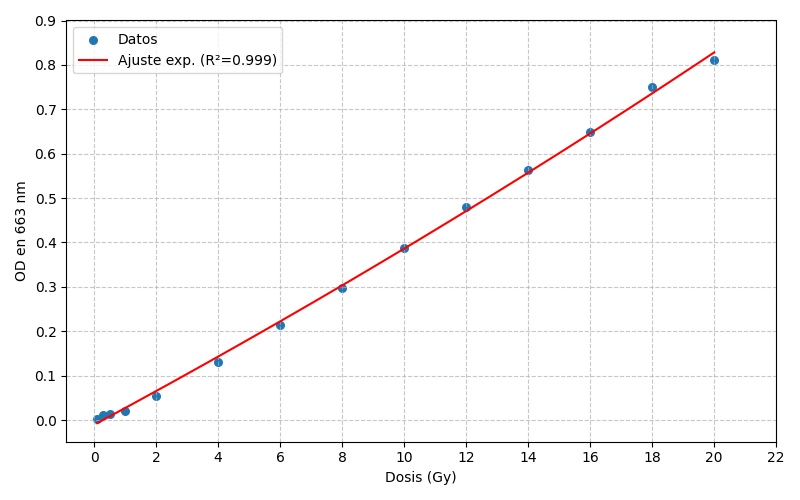
\includegraphics[width=\textwidth]{img_Esp/663Calib.png}
        \caption{Descripción imagen 2}
        \label{fig:img2}
    \end{subfigure}
    \caption{Título general para ambas imágenes}
    \label{fig:ambas}
\end{figure}




\section{Conclusiones}
Por que una radiocromica ouede sacae 3d y por que un fotodidodo es mas preciso, 
el uso de radiocromicas no es del todo bueno para estudios de bajas ni de altas dosis(flash), por un lado son imprecisas y por el otro se saturan. 
\bibliographystyle{plain} % Estilo de bibliografía
\bibliography{sample}
\end{document}












